\documentclass[twocolumn,twoside,11pt,a4paper]{article}

\usepackage[portuguese]{babel}  % portuguese
\usepackage{graphicx}           % images: .png or .pdf w/ pdflatex; .eps w/ latex


%% For iso-8859-1 (latin1), comment next line and uncomment the second line
\usepackage[utf8]{inputenc}
%\usepackage[latin1]{inputenc}

\usepackage[T1]{fontenc}        % T1 fonts
\usepackage{lmodern}            % fonts
\usepackage[sc]{mathpazo}       % Use the Palatino font
\linespread{1.05}               % Line spacing - Palatino needs more space between lines
\usepackage{microtype}          % Slightly tweak font spacing for aesthetics
\usepackage{url}                % urls
\usepackage[hang, small, labelfont=bf,up,textfont=it,up]{caption} % Custom captions under/above floats in tables or figures
\usepackage{booktabs}           % Horizontal rules in tables
\usepackage{float}              % Required for tables and figures in the multi-column environment - they need to be placed in specific locations with the [H] (e.g. \begin{table}[H])
\usepackage{paralist}           % Used for the compactitem environment which makes bullet points with less space between them

% geometry package
\usepackage[outer=20mm,inner=20mm,vmargin=15mm,includehead,includefoot,headheight=15pt]{geometry}
%% space between columns
\columnsep 10mm

\usepackage{abstract}           % Allows abstract customization
\renewcommand{\abstractnamefont}{\normalfont\bfseries} % Set the "Abstract" text to bold
\renewcommand{\abstracttextfont}{\normalfont\small\itshape} % Set the abstract itself to small italic text

% \usepackage{titlesec}           % Allows customization of titles
% \renewcommand\thesection{\Roman{section}} % Roman numerals for the sections
% \renewcommand\thesubsection{\Roman{subsection}} % Roman numerals for subsections
% \titleformat{\section}[block]{\large\scshape\centering}{\thesection.}{1em}{} % Change the look of the section titles
% \titleformat{\subsection}[block]{\large}{\thesubsection.}{1em}{} % Change the look of the section titles

\usepackage[pdftex]{hyperref}
\hypersetup{%
    a4paper = true,              % use A4 paper 
    bookmarks = true,            % make bookmarks 
    colorlinks = true,           % false: boxed links; true: colored links
    pdffitwindow = false,        % page fit to window when opened
    pdfpagemode = UseNone,       % do not show bookmarks
    pdfpagelayout = SinglePage,  % displays a single page
    pdfpagetransition = Replace, % page transition
    linkcolor=blue,              % hyperlink colors
    urlcolor=blue,
    citecolor=blue,
    anchorcolor=green
}

\usepackage{indentfirst}         % indent also 1st paragraph

\usepackage{fancyhdr}            % Headers and footers
\pagestyle{fancy}                % pages have headers and footers
\fancyhead{}                     % Blank out the default header
\fancyfoot{}                     % Blank out the default footer
\fancyhead[LO,RE]{Exploracafora} % Custom header text
\fancyhead[RO,LE]{\thepage}      % Custom header text
\fancyfoot[RO,LE]{Grupo 08, \today} % Custom footer text
\renewcommand{\headrulewidth}{0.4pt}
\renewcommand{\footrulewidth}{0.4pt}

%\hyphenation{}                  % explicit hyphenation

%----------------------------------------------------------------------------------------
%	macro definitions
%----------------------------------------------------------------------------------------

% entities
\newcommand{\class}[1]{{\normalfont\slshape #1\/}}
\newcommand{\svg}{\class{SVG}}
\newcommand{\scada}{\class{SCADA}}
\newcommand{\scadadms}{\class{SCADA/DMS}}

%----------------------------------------------------------------------------------------
%	TITLE SECTION
%----------------------------------------------------------------------------------------

\title{\vspace{-15mm}\fontsize{24pt}{10pt}\selectfont\textbf{Exploracafora}} % Article title

\author{Luís Pinto\\
\small \texttt{ei12108@fe.up.pt}\\
\and
Miguel Nunes\\
\small \texttt{ei12032@fe.up.pt}\\
\and
Rui Andrade\\
\small \texttt{ei12010@fe.up.pt}
\vspace{-5mm}
}

\date{\today}

%----------------------------------------------------------------------------------------

\begin{document}

\maketitle
\thispagestyle{plain}            % no headers in the first page

%----------------------------------------------------------------------------------------
%	ABSTRACT
%----------------------------------------------------------------------------------------

\begin{abstract}
Exploracafora é uma aplicação web que visa a exploração do mapa de Portugal e da sua fauna e flora. O mapa começa encoberto e vai aparecendo à medida que o utilizador se desloca pelo terreno português conectado à aplicação através do seu telemóvel. No mapa é exibida informação sobre espécies existentes. A aplicação recorre a um conjunto de serviços do portal iGEO para obter as espécies que existem em cada região do mapa, Google Maps mostrar o mapa e uma API do portal GBIF para obter informação mais detalhada sobre cada espécie.
\end{abstract}

%----------------------------------------------------------------------------------------
%	ARTICLE CONTENTS
%----------------------------------------------------------------------------------------

\section{Introdução}\label{sec:intro}
O projeto tem como objetivo o desenvolvimento de uma aplicação web que permite a exploração dinâmica de espécies de fauna e flora no território português. O desenvolvimento desta aplicação é motivado pela aprendizagem e descoberta dos diferentes elementos da natureza e do terreno português.
Para além desta introdução, onde se caracterizou o problema abordado por este projeto, refere-se na Secção ~\ref{sec:sota} o estado da arte e são descritas aplicações que abordam a mesma temática e as tecnologias a utilizar. Na Secção ~\ref{sec:application} está descrita com mais detalhe a aplicação a desenvolver. Na Secção ~\ref{sec:datamodel} são abordadas as fontes de dados a utilizar para obter as diversas informações necessárias para representar o mapa e mostrar toda a informação sobre os seres vivos presentes na aplicação. De seguida na Secção ~\ref{sec:metod} está presente a metodologia a seguir no desenvolvimento do projeto. Na Secção ~\ref{sec:requisitos} estão presentes os requisitos de utilizador levantados. A seguir, na secção ~\ref{sec:arquitetura} apresenta-se a aquitetura do projeto com identificação do fluxo de comunicação entre as diversas tecnologias utilizadas.

%------------------------------------------------

\section{Estado da arte}\label{sec:sota}

Existem várias aplicações que permitem a pesquisa de vários tipos de animais ou de plantas. Normalmente estas aplicações mostram informação de uma dada espécie depois do utilizador introduzir o nome comum ou cientifico do animal que procura. Outras aplicações permitem a descoberta de animais exibindo fotografias com informação anexada dos animais. Estas aplicações focam-se normalmente em contextos como animais raros, marinhos, extintos, voadores, etc. Como exemplo destas aplicações existe a Species Explorer~\cite{speciesexplorer} e a Rare Species Explorer~\cite{rarespecies}.

Existem também aplicações dedicadas exclusivamente à descoberta do mapa do mundo, utilizando o mesmo mecanismo presente na Exploracafora, começando com o mapa encoberto e descobrir à medida que o utilizador viaja pelo mundo. Um exemplo dessas aplicações é a Umbra.~\cite{umbra}

A aplicação desenvolvida tem como âmbito os seres vivos existentes no território português e ao contrário das aplicações existentes, esta foca-se na exploração, ou seja, o utilizador é convidado a viajar por Portugal para que possa explorar e ter conhecimento das espécies existentes em cada região, tornado assim a aquisição de conhecimento mais interativa e dinâmica.

Para desenvolver o trabalho escolheu-se PostgreSQL~\cite{postgresql} com a extensão Postgis~\cite{postgis} para a base de dados, pois facilita a representação de informação geográfica. Esta extensão permite por exemplo guardar as localizações de cada espécie na forma de polígonos e obter as localizações que contêm um dado ponto geográfico, como a localização do utilizador. Sendo uma aplicação web para dispositivos móveis, desenvolvemos a interface com HTML5, CSS3, Bootstrap e javascript. O servidor é implementado em Nodejs~\cite{nodejs} por ser uma tecnologia bastante utilizada atualmente e pelo interesse do grupo em experimentá-la.

%------------------------------------------------

\section{Exploracafora}\label{sec:application}

A Exploracafora é uma aplicação que permite conjugar a visualização do mapa português com a interatividade de um jogo de exploração. Na aplicação existe um mapa no qual o utilizador observa a sua posição e tudo aquilo que o rodeia dentro de um raio pré-definido. À medida que a pessoa começa a deslocar-se o mapa vai mostrando todos os pontos importantes. No início do uso da aplicação todo o mapa encontra-se encoberto e é desvendado à medida que novas áreas são exploradas. Deste modo a aplicação torna-se interativa e dinâmica como se de um jogo se tratasse.

O utilizador poderá encontrar na aplicação informação sobre plantas, insetos, aranhas, bivalves, gastrópodes, peixes, anfíbios, répteis e mamíferos existentes em Portugal. 

\section{Fontes de dados}\label{sec:datamodel}
Utilizam-se várias fontes para reunir toda a informação necessária. São usados serviços do portal iGEO (informação Geográfica) para obter as espécies existentes num dado ponto de Portugal, estes serviços indicam para cada ser vivo as regiões de Portugal onde estes existem.~\cite{igeo} Essas regiões são definidas por vértices de polígonos com coordenadas GPS. Desenvolveu-se um pequeno programa em java que recolhe toda a informação de cada serviço do portal iGEIO em XML e através da utilização de JDOM, para interpretar as respostas, gera um ficheiro com as instruções necessárias para introduzir os dados na base de dados em SQL. Apresenta-se na figura \ref{fig:localizacoes} o modelo de dados utilizado na base de dados SQL. 

\begin{figure}[ht!]
	\begin{center}
		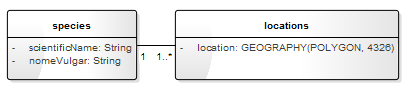
\includegraphics[width=0.50\textwidth]{localizacao_especies}
		\caption{Modelo de dados das espécies e respetivas localizações}
		\label{fig:localizacoes}
	\end{center}
\end{figure} 


O modelo de dados das respostas do portal iGEO é apresentado na figura \ref{fig:igeo}. Consiste numa coleção de elementos que contêm o nome científico e vulgar, o id e as regiões do mapa, conjunto de coordenadas GPS que definem um polígono, onde estas estão presentes.

\begin{figure}[ht!]
	\begin{center}
		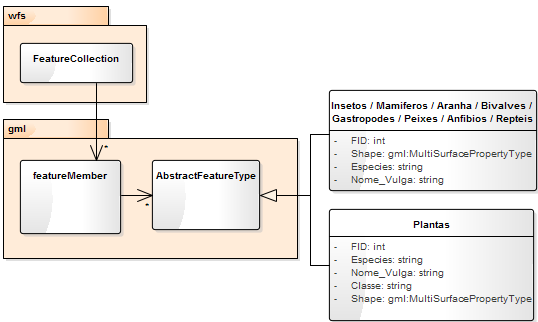
\includegraphics[width=0.50\textwidth]{igeo}
		\caption{Modelo de dados dos serviços do portal iGEO}
		\label{fig:igeo}
	\end{center}
\end{figure} 


Em complementaridade com estes serviços recorre-se a uma API do site GBIF (Global Biodiversity Information Facility) para obter informação mais detalhada sobre cada espécie, como reino, família, imagens, etc.~\cite{gbif} Esta API reúne informação de diversas fontes, contendo no momento informação sobre aproximadamente 1,650,00 espécies. Por fim é necessário recorrer ao Google Maps para mostrar o mapa de Portugal e toda a informação a ele associada.~\cite{googlemaps}

	O modelo de dados da API GBIF depende do serviço utilizado. Pretende-se utilizar o serviço de pesquisa pelo nome científico de um ser vivo, que devolve um conjunto de registos sobre a espécie pesquisada, o modelo está representado na figura  \ref{fig:scientName}. No caso de se obter um registo com uma referência para a página da Wikipédia, pretende-se utilizar a chave dessa referência para obter o conteúdo multimédia, tipicamente uma imagem, utilizada nessa mesma página para identificar o ser vivo e ainda obter a descrição inicial. O modelo das respostas ao conteúdo multimédia e à descrição do servivo estão presentes na imagem \ref{fig:multimedia} e na imagem \ref{fig:descricao}, respetivamente.

\begin{figure}[ht!]
	\begin{center}
		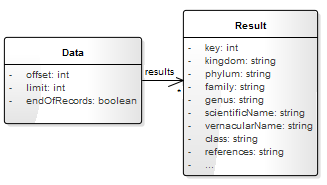
\includegraphics[width=0.50\textwidth]{Scientify_name}
		\caption{Modelo da pesquisa por nome científico}
		\label{fig:scientName}
	\end{center}
\end{figure} 

\begin{figure}[ht!]
	\begin{center}
		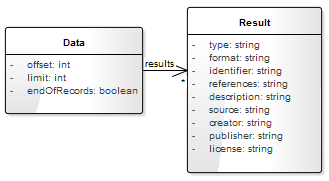
\includegraphics[width=0.50\textwidth]{Search_image}
		\caption{Modelo da resposta  para obter a imagem do animal na Wikipédia}
		\label{fig:multimedia}
	\end{center}
\end{figure} 

\begin{figure}[ht!]
	\begin{center}
		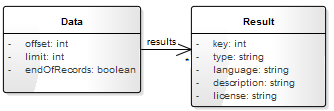
\includegraphics[width=0.50\textwidth]{description}
		\caption{Formato da resposta para obter a descrição do animal da página da Wikipédia}
		\label{fig:descricao}
	\end{center}
\end{figure} 

Na base de dados pretende-se ainda guardar os percursos que o utilizar percorreu, para isso representa-se o mapa como uma grelha, com um valor binário a indicar se o utilizador já esteve em cada célula da grelha. O modelo de dados é apresentado na figura  \ref{fig:userdata}.

\begin{figure}[ht!]
	\begin{center}
		\leavevmode
		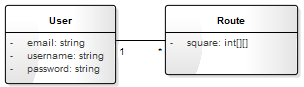
\includegraphics[width=0.45\textwidth]{userdata}
		\caption{Modelo de dados para guardar a informação dos percursos do utilizador}
		\label{fig:userdata}
	\end{center}
\end{figure} 



%------------------------------------------------

\section{Metodologia}\label{sec:metod}
A construção do projeto está dividida em várias etapas: a análise do formato dos dados das múltiplas fontes, a decisão do tipo de armazenamento e processamento dos dados, a identificação de requisitos e tecnologias a utilizar, a elaboração da arquitetura e desenvolvimento de código final da aplicação e dos web services da nossa API.

%------------------------------------------------

\section{Requisitos}\label{sec:requisitos}
De modo a satisfazer todas as necessidades do utilizador final e garantir que todas as funcionalidades são apresentadas de forma explícita, serão apresentados os requisitos, na primeira pessoa, que a aplicação deve disponibilizar ao utilizador.
 Como utilizador quero ver as espécies que existem perto da minha localização, visualizar áreas já exploradas por mim, ver toda a informação acerca de uma espécie, poder procurar no mapa áreas onde se encontra certa fauna ou flora e ter acesso a um catálogo com todas as espécies descobertas e por descobrir.
	A aplicação web vai necessitar de internet e serviços de localização para que possa funcionar nas condições normais. 

%------------------------------------------------

\section{Arquitetura}\label{sec:arquitetura}
A arquitetura é constituída por um servidor que vai comunicar com as diferentes APIs. Para a base de dados foi escolhido o PostGIS, que é uma base de dados espacial estendida do PostgreSQL, na qual são suportados objetos geográficos que permitem a ocorrência de perguntas de localização em SQL. Para implementação do mapa, é usado os serviços do Google Maps e como fonte de informação para as espécies será usado a API do GBIF (Global Biodiversity Information Facility). O esquema da arquitetura é apresentado na figura \ref{fig:arq}.

\begin{figure}[ht!]
	\begin{center}
		\leavevmode
		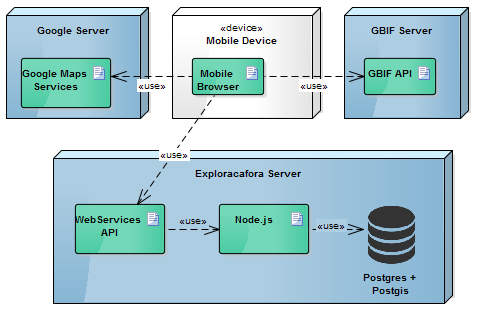
\includegraphics[width=0.50\textwidth]{Deployment_Model}
		\caption{Esquema da arquitetura}
		\label{fig:arq}
	\end{center}
\end{figure} 



%------------------------------------------------

\section{Conclusão}\label{sec:conclusions}
Neste artigo apresentou-se o tema e funcionalidades da aplicação final, as fontes de dados que são usadas, os requisitos finais, as tecnologias utilizadas e ainda a forma como interagem. Para validar a arquitetura desenhada e tecnologias escolhidas foi implementado um pequeno protótipo da aplicação Exploracafora. 


%----------------------------------------------------------------------------------------
%	REFERENCE LIST
%----------------------------------------------------------------------------------------

%% auto bibliographic list 
\renewcommand{\bibname}{Referências}
% uses bibtex file
%\bibliographystyle{alpha-pt}
%\bibliographystyle{alpha}
\bibliographystyle{unsrt-pt}
%\bibliographystyle{unsrt}
\bibliography{artigo}

%----------------------------------------------------------------------------------------

\end{document}


